\documentclass[a4paper]{article}
\usepackage[spanish]{babel}
\usepackage[utf8]{inputenc}
\usepackage{graphicx}
\usepackage{pdfpages}
\usepackage{enumerate}
\usepackage{listings}
\usepackage{color}
\usepackage{indentfirst}
\usepackage{fancyhdr}
\usepackage{latexsym}
\usepackage[colorlinks=true, linkcolor=black]{hyperref}
%\usepackage{makeidx}
%\usepackage{float}
\usepackage{wrapfig}
\usepackage{calc}
\usepackage{amsmath, amsthm, amssymb}
\usepackage{amsfonts}
%\lstset{language=C}
\definecolor{gray}{gray}{0.5}
\definecolor{light-gray}{gray}{0.95}
\definecolor{orange}{rgb}{1,0.5,0}

\usepackage{fancyhdr}
\pagestyle{fancy}

%\renewcommand{\chaptermark}[1]{\markboth{#1}{}}
\renewcommand{\sectionmark}[1]{\markright{\thesection\ - #1}}

\fancyhf{}

\fancyhead[LO]{Sección \rightmark} % \thesection\
\fancyfoot[LO]{\small{Raul Benitti, Damián Castro, Leandro Matayoshi, Javier San Miguel}}
\fancyfoot[RO]{\thepage}
\renewcommand{\headrulewidth}{0.5pt}
\renewcommand{\footrulewidth}{0.5pt}
\setlength{\hoffset}{-0.8in}
\setlength{\textwidth}{16cm}
%\setlength{\hoffset}{-1.1cm}
%\setlength{\textwidth}{16cm}
\setlength{\headsep}{0.5cm}
\setlength{\textheight}{25cm}
\setlength{\voffset}{-0.7in}
\setlength{\headwidth}{\textwidth}
\setlength{\headheight}{13.1pt}

\renewcommand{\baselinestretch}{1.1}  % line spacing


% \setcounter{secnumdepth}{2}
\usepackage{underscore}
\usepackage{caratula}
\usepackage{url}
\usepackage{float}
\usepackage[noend]{algpseudocode}
\usepackage{minted}

\newcommand{\cod}[1]{{\tt #1}}
\newcommand{\negro}[1]{{\bf #1}}
\newcommand{\ital}[1]{{\em #1}}
\newcommand{\may}[1]{{\sc #1}}
\newcommand{\tab}{\hspace*{2em}}

\hypersetup{
 pdfstartview= {FitH \hypercalcbp{\paperheight-\topmargin-1in-\headheight}},
 pdfauthor={Grupo},
 pdfsubject={Dise\~{n}o}
}

\lstset { %
    language=C++,
    backgroundcolor=\color{black!5}, % set backgroundcolor
    basicstyle=\footnotesize,% basic font setting
}

\lstset{escapechar=@}


\begin{document}

\thispagestyle{empty}
\materia{Bases de Datos}
\submateria{Segundo Cuatrimestre de 2015}
\titulo{Trabajo Práctico II: Bases de datos NoSql}
%\subtitulo{Scheduling}
\integrante{Raul Benitti}{592/08}{raulbenitti@gmail.com }
\integrante{Damian Castro}{326/11}{ltdicai@gmail.com }
\integrante{Leandro Matayoshi}{79/11}{leandro.matayoshi@gmail.com }
\integrante{Javier San Miguel}{786/10}{javiersm00@gmail.com}

\makeatletter

\maketitle

\newpage
\section{Introducción}

En el presente trabajo desarrollaremos un acercamiento práctico a las bases de datos NoSQL.
Para tal fin utilizaremos MongoDB, una base de datos de documentos, y revisaremos tres puntos básicos de uso:
\begin{itemize}
\item Implementación de un modelo conceptual, guiado por las consultas directas que se desean realizar sobre los datos.
\item Implementación de consultas por medio de MapReduce, uno de las tecnologías estandarte de las bases de datos orientadas a documento
\item Implementación de escalado horizontal, conocido como sharding.
\end{itemize}
Como último punto, desarrollaremos brevemente como cambiarían las soluciones implementadas en MongoDB si se utilizara una base de datos de tipo
Key-Value.


\newpage
\section{Modelo}

\subsection{Empleados que atendieron clientes mayores de edad}

\begin{listing}
\begin{minted}[frame=single,
               framesep=3mm,
               linenos=true,
               xleftmargin=21pt,
               tabsize=4]{js}
{
  "_id" : ObjectId("5622bf41228da935bd5e0a6a"),
  "nroLegajo" : 234,
  "nombre" : "Pepito Suarez",
  "clientes_mayores" : [
    {
      "_id" : ObjectId("5622c1d3228da935bd5e0a6b"),
      "fecha" : ISODate("2015-10-01T00:00:00Z")
    }
  ],
  "clientes_menores" : [ ],
  "sectores" : [
    {
      "sector" : "Comestibles",
      "tarea" : "Gerente"
    },
    {
      "sector" : "Indumentaria deportiva",
      "tarea" : "Supervisor"
    }
  ]
}
\end{minted}
\caption{Ejemplo Empleado}
\label{json-example}
\end{listing}

\textbf{Consulta: } db.empleados.find(\{``clientes_mayores": \{\$exists: true, \$not: \{\$size: 0\}\}\})

\vspace{3em}

\subsection{Artículos más vendidos}
\begin{listing}
\begin{minted}[frame=single,
               framesep=3mm,
               linenos=true,
               xleftmargin=21pt,
               tabsize=4]{js}
{
  "_id" : ObjectId("5622d234228da935bd5e0a6f"),
  "codBarras" : 342391,
  "nombre" : "Pro Speed Z-7",
  "sector" : "Calzado",
  "cant_unidades_vendidas" : 0
}
\end{minted}
\caption{Ejemplo Artículo}
\label{json-example}
\end{listing}

\textbf{Consulta: }
\begin{enumerate}
  \item max_cant_unidades_vendidas = (db.articulos.aggregate([\{\$group : \{_id: null, max : \{\$max : ``\$cant_unidades_vendidas"\}\}\}])).next().max
  \item db.articulos.find(``cant_unidades_vendidas" : max_cant_unidades_vendidas)
\end{enumerate}

\vspace{3em}

\subsection{Sectores donde trabajan exactamente 3 empleados}
\begin{listing}
\begin{minted}[frame=single,
               framesep=3mm,
               linenos=true,
               xleftmargin=21pt,
               tabsize=4]{js}
{
  "_id" : ObjectId("5622df91228da935bd5e0a75"),
  "codSector" : "Comestibles",
  "empleados" : {
    "total" : 1,
    "lista" : [ ObjectId("5622bf41228da935bd5e0a6a") ]
  }
}
\end{minted}
\caption{Ejemplo Sector}
\label{json-example}
\end{listing}

\textbf{Consulta: } db.sectores.find(\{``empleados.lista": \{\$size: 3\}\})

\vspace{3em}

\subsection{Empleado que trabaja en más sectores}

\

\textbf{Consulta: }

\begin{enumerate}
  \item var max = db.empleados.aggregate([\{\$group: \{\_id:null, max: \{\$max: \{\$size: ``\$sectores"\}\}\}\}]).next().max
  \item db.empleados.find(\{sectores: \{\$size: max\}\})
\end{enumerate}

\vspace{3em}

\subsection{Ranking de los clientes con mayor cantidad de compras (total de unidades)}

\begin{listing}
\begin{minted}[frame=single,
               framesep=3mm,
               linenos=true,
               xleftmargin=21pt,
               tabsize=4]{js}
{
  "_id" : ObjectId("5622c1d3228da935bd5e0a6b"),
  "dni" : 28012849,
  "nombre" : "Julio Jericho",
  "edad" : 23,
  "articulos" : {
    "total" : 4,
    "lista" : [ {"id": ObjectId("ff20ef41228da935bd5583bd"), "cantidad": 3},
                {"id": ObjectId("4729bce098bbddee98100acc"), "cantidad": 1}
              ]
  }
}

\end{minted}
\caption{Ejemplo Cliente}
\label{json-example}
\end{listing}

Cuando el cliente compra una cantidad determinada de un producto, se agrega una nueva entrada al
final del arreglo \emph{lista}, sumando al valor de total la cantidad de unidades compradas

\vspace{3em}

\subsection{Cantidad de compras realizadas por clientes de la misma edad}

\textbf{Consulta: }

db.clientes.aggregate([\{\$project: \{``art_total": ``\$articulos.total", ``edad": 1\}\}, \{\$group: \{_id: ``\$edad", total: \{ \$sum: ``\$art_total"\}\}\}])
















\newpage
\section{MapReduce}

\subsection{Cantidad de disposiciones de tipo resoluciones realizadas en Abril del 2013}

Por cada disposición, si cumple con las restricciones emitimos como clave: ``Resoluciones", y
1 como valor. El reduce consiste simplemente en la suma de todos los values.

\begin{lstlisting}
var m = function(){
  var date = convertDate(this.FechaDisposicion);
  if(date){
    var month = date.getMonth();
    if (month == 3 && this.Tipo == "Resoluciones"){
      emit(this.Tipo, 1);
    }
  }
}

var r = function(key,values) {
    return Array.sum(values)
}

printjson(db.disposiciones.mapReduce(m,r,{out: {inline: 1},
          scope: {convertDate: convertDate}}));
\end{lstlisting}

\vspace{4em}

\subsection{Cantidad de disposiciones por tipo definido}

Este caso consiste en un agrupamiento por ``Tipo" con la suma de la cantidad de documentos
como valor. Por lo tanto, la clave en este caso es el tipo de la disposición. Al igual que
en el caso anterior, se emite 1 como valor por cada documento y al reducir se suman todos
los valores.

\begin{lstlisting}
var m = function(){
  if (this.Tipo != ""){
    emit(this["Tipo"], 1);
  }
}
var r = function(key, values) {
  return Array.sum(values);
}

printjson(db.disposiciones.mapReduce(m,r,{out: {inline: 1}}));
\end{lstlisting}

\subsection{Fecha más citada para todos los informes}

Utilizamos la función convertDate para transformar las distintas fechas a un formato
común. Las fechas se presentan como day-month-year, day/month/year o en formato iso:
2015-11-21T01:51:17Z.

Las claves son las fechas normalizadas, y emitimos 1 como valor tanto por la \emph{FechaBOJA}
como por la \emph{FechaDisposicion}.

\begin{lstlisting}

var m = function(){
  var fecha_boja = convertDate(this.FechaBOJA);
  var fecha_disp = convertDate(this.FechaDisposicion);
  if (fecha_boja){
    emit(fecha_boja, 1);
  }
  if(fecha_disp){
    emit(fecha_disp, 1);
  }
}
var r = function(key, values) {
  return Array.sum(values);
}


var res = db.disposiciones.mapReduce(m,r,{out: {inline: 1},
                                    scope: {convertDate: convertDate}})
printjson(res);

//Find max
var max = null;
for(var idx = 0; idx < res.results.length; ++idx){
  var item = res.results[idx];
  if(max){
    if (Math.max(max.value, item.value) != max.value) max = item;
  }
  else{
    max = item;
  }
}

printjson(max);

\end{lstlisting}

\subsection{Devolver la mayor cantidad de páginas utilizadas por cada tipo de disposición}

La consulta consiste en un agrupamiento sobre tipo de disposición
con agregación sobre el máximo de las páginas utilizadas.

Por lo tanto emitimos el tipo de documento como clave y la cantidad de páginas utilizadas
como valor. El reduce encuentra el máximo sobre la lista de valores.

\begin{lstlisting}
var m = function(){
  var pagina_inicial = this["PaginaInicial"],
    pagina_final = this["PaginaFinal"];
  emit(this["Tipo"], pagina_final - pagina_inicial)
}

var r = function(key, values){
  var max = 0;
  // Calculo del maximo
  for(var i = 0; i < values.length; ++i){
    if (values[i] > max){
      max = values[i];
    }
  }
  return max;
}

var res = db.disposiciones.mapReduce(m, r, {out: {inline: 1}})
printjson(res);
\end{lstlisting}

\subsection{Función para convertir las fechas}

\begin{lstlisting}
function convertDate(str){
  if(str == "") return null;
  if(/^\d{4}-\d{2}-\d{2}T\d{2}:\d{2}:\d{2}Z?$/.test(str)){
    return new Date(str.replace(/^00/, "20"));
  }
  else if(/^\d{2}[-\/]\d{2}[-\/]\d{4}$/.test(str)){
    var parts = str.split(/[-\/]/);
    var aux = parts[0];
    parts[0] = parts[2];
    parts[2] = aux;
    return new Date(parts.join("-"));
  }
  else{
    return null;
  }
}
\end{lstlisting}






\newpage
\section{Sharding}

El objetivo de esta sección es analizar la distribución de la carga en una colección repartida entre varios shards.

La estructura de los documentos es la siguiente:

\begin{listing}
\begin{minted}[frame=single,
               framesep=3mm,
               linenos=true,
               xleftmargin=21pt,
               tabsize=4]{js}
{
  "nombre": nombrePersona
  "password": passwordPersona
  "codigo_postal": getRandomIntInclusive(1, 1000000),
  "genero": generoPersona,
  "edad": edadPersona
  "fecha_creacion": fechaCreacion
}

\end{minted}
\caption{Ejemplo persona}
\label{json-example}
\end{listing}

La shard key se establece a partir del atributo \emph{codigo\_postal}, generado de forma pseudoaleatoria.
Los documentos son agregados en bloques de 20.000 documentos, hasta alcanzar un total de 500.000. El tamaño
total de la colección es aproximadamente 115 MB. Esto genera un total de 25 mediciones por experimento.

Es posible generar los shards de 2 formas posibles sobre la shard key:
\begin{itemize}
\item Por rango
\item Por hash
\end{itemize}

Por cada uno de estos tipos realizamos un experimento con 2 y 3 shards.

\subsection{Partición basada en rango}

\begin{figure}[!h]
  \begin{center}
      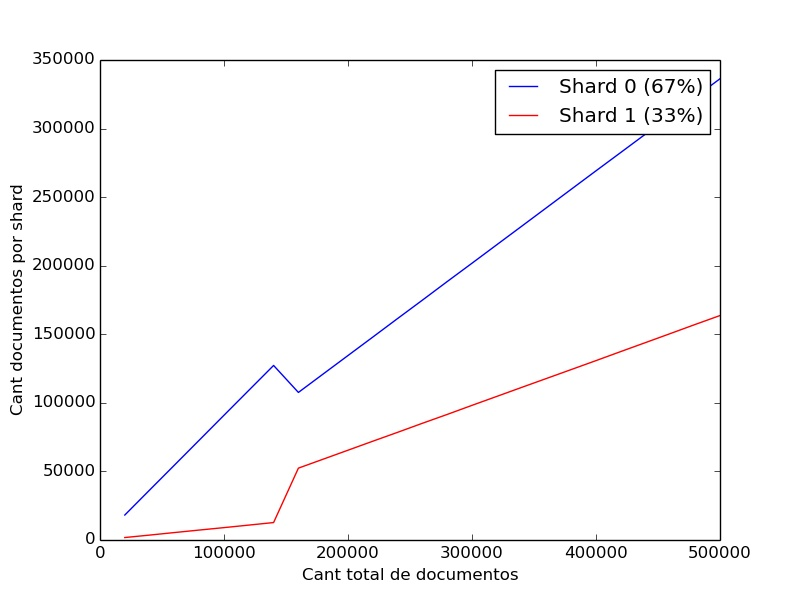
\includegraphics[scale=0.4]{imagenes/range1.jpg}
      \caption{2 Shards utilizando partición de keys por rango}
      \label{fig:contra1}
  \end{center}
\end{figure}

~

La carga no se reparte uniformemente. El shard 0 mantiene un aproximadamente un 67\% de los datos a lo largo de todo
el experimento, mientras que el segundo shard mantiene el 33\% de los datos.

\begin{figure}[!h]
  \begin{center}
      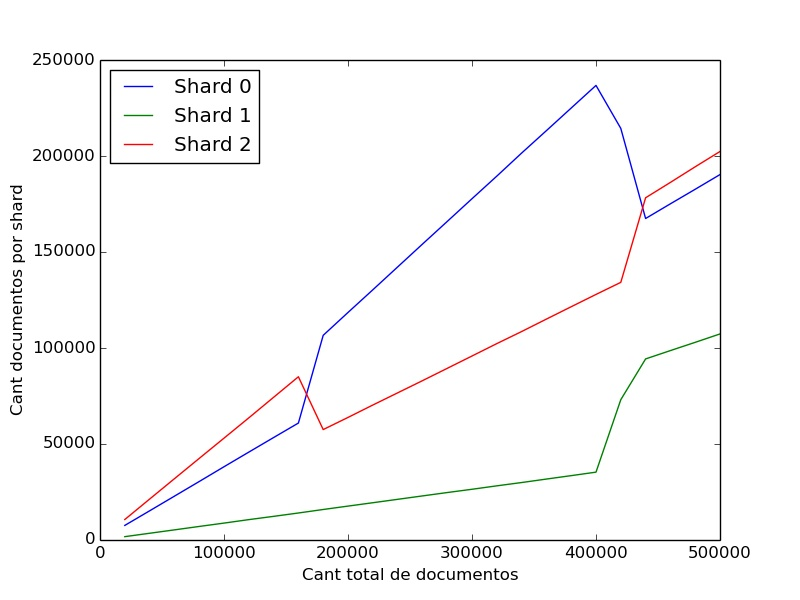
\includegraphics[scale=0.4]{imagenes/range2.jpg}
      \caption{3 Shards utilizando partición de keys por rango}
      \label{fig:contra1}
  \end{center}
\end{figure}

~

La existencia de un tercer shard favorece al balance de la carga, aunque sigue habiendo un shard que contiene
pocos datos.

\subsection{Partición basada en hash}

\begin{figure}[!h]
  \begin{center}
      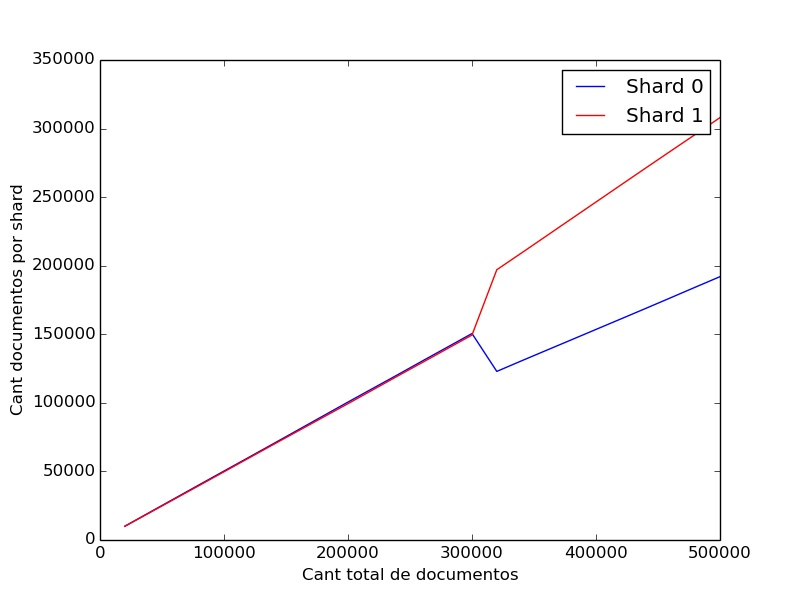
\includegraphics[scale=0.4]{imagenes/hash1.jpg}
      \caption{2 Shards utilizando partición de keys basada en hash}
      \label{fig:contra1}
  \end{center}
\end{figure}

~

La carga se distribuye de manera uniforme hasta un punto de quiebre, en donde un shard queda con más carga que
el otro.

\begin{figure}[!h]
  \begin{center}
      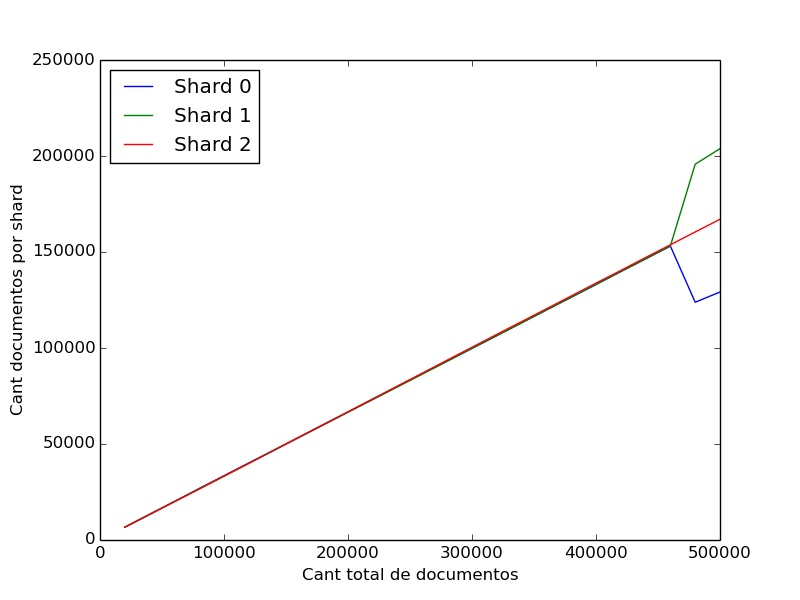
\includegraphics[scale=0.4]{imagenes/hash2.jpg}
      \caption{3 Shards utilizando partición de keys basada en hash}
      \label{fig:contra1}
  \end{center}
\end{figure}

~

Nuevamente, la existencia de un tercer shard aporta estabilidad al balanceo. En este caso, la distribución
se mantiene uniforme casi hasta el final de la experimentación. En dicho punto, los shards quedan
con una distribución levemente diferente.

~

\subsection{Conclusión}

Para valores de shard keys generados de forma pseudoaleatoria es conveniente tener una clustering key
basada en hash para mantener el balanceo uniforme por sobre una con rango.
La existencia de mayor cantidad de shards favorecen a la uniformidad de la distribución.



\newpage
\section{Key-Value como alternativa}

\subsection{General}
Elegimos ejemplificar los cambios que implicaría utilizar una base de datos Key-Value.
Este tipo de bases está muy relaciono con las bases de datos Document, consideradas como una versión más potente de las primeras.
Ambas mantiene una _clave_ relacionada con un único _valor_, y esta relación define el límite de atomicidad. Además,
si bien en ambos tipos de bases de datos pueden modelarse relaciones entre entidades, la coherencia y validez de estas relaciones
deben ser mantenidad por el programador desde el código de la aplicación.

La diferencia fundamental entre ambos tipos radica en que, en las bases Key-Values, el _valor_ solo se considera como una cadena de bits
sin semántica, por lo que cualquier información que allí se guarde resulta inútil a fines de consulta y procesamiento directo: en una
base Key-Value, la única manera de acceder a un dato es sabiendo bajo que clave se almacena. En cambio, las bases de datos de documentos sí otorgan
una semántica a los valores relacionados a una clave - la idea de un documento con campos definidos. Esto les permite proveer operaciones
de búsqueda y agregación más cercanas a aquellas encontradas en bases de datos relacionales.

\subsection{Punto 1}
Como en las bases Key-Value no hay acceso posible a los datos si no se
especifican las claves, a diferencia del modelo realizado en Document DB, necesitamos mantener
información explícita sobre las claves de las entidades que vamos a almacenar. Por esto, utilizaríamos un bucket Claves con

~

  claves[``empleados"] $\rightarrow$ {[nroLegajo]}

  claves[``productos"] $\rightarrow$ {[codigoDeBarra]}

  claves[``sectores"]  $\rightarrow$ {[codigoSector]}

  claves[``clientes"]  $\rightarrow$ {[dni]}

~

Las bases Key-Value tampoco nos proveen métodos para operar sobre los valores almacenados por clave,
puesto que la parte del valor es considera como una caja negra. Por esto, si se quiere tener
una estructura de clave-valor que no sea extremadamente rigida (como sería el caso
de guardar claves-valores del estilo [``empleadosQueAtendieronAdultos"] $\rightarrow$ \{[nroLegajo]\}),
necesitamos poder iterar sobre las claves y operar con los valores por fuera de la base.

Por ejemplo, podriamos definir la siguiente estructura (incompleta) con los datos necesarios para las consultas requeridas:
\begin{enumerate}
\item empleados[$<nroLegajo>$:``clientes"] $\rightarrow$ \{``adultos": int, ``total": int, ``clientesAtendidos": [dni]\}
\item articulos[$<codigoDeBarra>$] $\rightarrow$ \{``cantidadVendida": int\}
\item sectores[$<codigoSector>$] $\rightarrow$ \{``cantidadEmpleados":int, ``empleados":[nroLegajo]\}
\item clientes[$<dni>$] $\rightarrow$ \{cantidadCompras: int\}
\item empleados[$<nroLegajo>$:``sectores"] $\rightarrow$ \{``cantidadSectores": int, ``sectores":[codigoSector]\}
\item clientes[``compras":$<edad>$] $\rightarrow$ {``cantidadCompras": int}
\end{enumerate}

Entonces, para responder la consulta ``Los empleados que atendieron clientes mayores de edad", el programador debería:

\begin{itemize}
\item conseguir los nroLegajo de los empleados utilizando claves[``empleados"]
\item para cada nroLegajo, obtener el json almacenado en empleados[$<nroLegajo>$:``clientes"]
\item mantener una lista de los empleados (nroLegajo) con mayor valor en el campo ``adultos" del json obtenido.
\end{itemize}

\subsection{Punto 2}
Como comentamos anteriormente, las bases de datos Key-Value no proveen métodos para realizar operaciones sobre la información almacenada
en los valores. Por lo tanto, el esquema de Map Reduce debería ser implementado en una capa superior, ya sea directamente por el programador o por una
librería. Si no existe una librería que provea tal servicio, podría resultar mas conveniente proceder
tal como lo haríamos para las consultas del punto 1.


\subsection{Punto 3}
El concepto de Sharding puede aplicarse de la misma manera tanto a bases Key-Value como Document, y deben tenerse en cuentas
las mismas consideraciones sobre la distribución de las claves elegidas para realizar las particiones. Existe, sin embargo, una diferencia
importante a considerar:
dependiendo de como se manejen los atributos de una entidad en Key-Value (agregados en una clave$\rightarrow$valores o desagregados en varias clave:atributo$\rightarrow$valor), pueden
darse casos en que una misma entidad tenga sus atributos repartidos entre distintos shards.



\newpage
\section{Conclusiones}

En el transcurso del desarrollo de este trabajo nos enfrentamos con problemas de diseño e implementación
típicos en el uso de bases NoSQL. Entre ellos:

\begin{itemize}
  \item Representar la información para prescindir del uso de join, tratando de mantener un balance entre
la consistencia de los datos y la atomicidad de las operaciones.
  \item  Extraer información
utilizando la técnica de MapReduce, en la cual el propio programador debe cumplir un rol que suele relegarse al motor de bases de dato relacionales
  \item Dividir de forma adecuada los datos a fin de lograr escalabilidad.
\end{itemize}

A partir de todo esto, llegamos a entender que las bases de datos NoSQL pueden ser muy útiles en situaciones particulares en las que, entre otras cosas:
\begin{itemize}
  \item Las consultas que se realizaran sobre los datos son prefijadas o predecibles
  \item No se requiera realizar consultas arbitrarias
  \item La consistencia de la informacion no es un factor relevante (aunque existen bases NoSQL que cumplen con ACID, no son la mayoría ni las más utilizadas)
  \item Se espera que el sistema deba procesar cantidades extremadamente grandes de información de manera eficaz
  \item Se espera que millones de usuarios utilicen el sistema de manera concurrente
\end{itemize}

Todas estas características no implican descartar el uso de bases de datos relaciones sino que, si dichas circunstancias están presente, permiten evaluar
la conveniencia de dejar de lado la complejidad en que incurren las bases relacionales que cumplen con las propiedades ACID por otras bases con una mecánica simplificada a costa de
no hacerlo.

En definitiva, las bases de datos NoSQL no vienen a reemplazar a las bases relacionales - las complementan, poniendo a disposición de los desarrolladores
más herramientas con las que encontrar soluciones eficaces a los problemas cada
vez más complejos con los que se enfrenta el mundo de la administración de información.


\newpage
\section{Apéndice}

\subsection{Status de los shardings}

Incluímos a continuación un fragmento de la salida de MongoDB al correr los comandos \emph{sh.status()}
y \emph{db.people.getShardDistribution()}:

\begin{listing}
\begin{minted}[
               framesep=3mm,
               linenos=true,
               xleftmargin=21pt,
               tabsize=4]{js}
{
  MongoDB shell version: 3.0.7
  connecting to: localhost:10003/admin
  Enabling sharding
  { "ok" : 0, "errmsg" : "already enabled" }
  --- Sharding Status ---
    sharding version: {
    "_id" : 1,
    "minCompatibleVersion" : 5,
    "currentVersion" : 6,
    "clusterId" : ObjectId("5655105adce14eebdfb2d003")
  }
    shards:
    {  "_id" : "shard0",  "host" : "localhost:10000" }
    {  "_id" : "shard1",  "host" : "localhost:10001" }
    balancer:
    Currently enabled:  yes
    Currently running:  no
    Failed balancer rounds in last 5 attempts:  0
    Migration Results for the last 24 hours:
      2 : Success
    databases:
    {  "_id" : "admin",  "partitioned" : false,  "primary" : "config" }
    {  "_id" : "sharding_test_hash",  "partitioned" : true,  "primary" : "shard0" }

  Create index hashed
  {
    "raw" : {
      "localhost:10000" : {
        "createdCollectionAutomatically" : true,
        "numIndexesBefore" : 1,
        "numIndexesAfter" : 2,
        "ok" : 1
      }
    },
    "ok" : 1
  }
}
\end{minted}
\caption{Standard output de MongoDB al momento de aplicar el sharding}
\label{json-example}
\end{listing}

\begin{listing}
\begin{minted}[
               framesep=3mm,
               linenos=true,
               xleftmargin=21pt,
               tabsize=4]{js}
{
  Use index as sharding key
  { "collectionsharded" : "sharding_test_hash.people", "ok" : 1 }
  Inserting 20000 entries

  Shard shard0 at localhost:10000
   data : 2.29MiB docs : 10025 chunks : 2
   estimated data per chunk : 1.14MiB
   estimated docs per chunk : 5012

  Shard shard1 at localhost:10001
   data : 2.28MiB docs : 9975 chunks : 2
   estimated data per chunk : 1.14MiB
   estimated docs per chunk : 4987

  Totals
   data : 4.57MiB docs : 20000 chunks : 4
   Shard shard0 contains 50.12
   Shard shard1 contains 49.87
}
\end{minted}
\caption{db.people.getShardDistribution() luego de insertar los primeros 20000(2 shards)}
\label{json-example}
\end{listing}



\thispagestyle{empty}
\vfill

\thispagestyle{empty}
\vspace{3cm}
%\tableofcontents
\newpage

\newenvironment{myindentpar}[1]
{\begin{list}{1}
         {\setlength{\leftmargin}{#1}}
         \item[]
}
{\end{list} }

%\normalsize
\newpage

% -------------------------------------------------------
% DER
% -------------------------------------------------------
\newpage


\bibliographystyle{plain}
\bibliography{tp3}

\end{document}
